\documentclass[conference]{IEEEtran}

\usepackage{cite}
\usepackage{amsmath,amssymb,amsfonts}
\usepackage{algorithmic}
\usepackage{graphicx}
\usepackage{textcomp}
\usepackage{xcolor}
\usepackage{hyperref}
\usepackage{multirow}
\usepackage{booktabs}
\usepackage{caption}
\usepackage{float}



\graphicspath{{src/}}

\def\BibTeX{{\rm B\kern-.05em{\sc i\kern-.025em b}\kern-.08em
    T\kern-.1667em\lower.7ex\hbox{E}\kern-.125emX}}
\begin{document}

\title{A Comparative Study of Apache Spark and Ray for
Scalable Big Data Analytics and Machine Learning in Python}

\author{
    
  \IEEEauthorblockN{Kolydakis Emmanouil}
  \IEEEauthorblockA{\textit{Electrical \& Computer Engineering} \\
  \textit{National Technical University of Athens}\\
  Athens, Greece \\
  03120156}
  \and
  \IEEEauthorblockN{Kouriannidis Iasonas}
  \IEEEauthorblockA{\textit{Electrical \& Computer Engineering} \\
  \textit{National Technical University of Athens}\\
  Athens, Greece \\
  03120439}

}

\maketitle

\begin{abstract}
As data-intensive applications become more prevalent, the need for
efficient and scalable big data processing frameworks has never been greater.
This work presents a comparative analysis of two prominent distributed systems, Apache Spark and
Ray, focusing on their performance in executing Extract, Transform, Load (ETL) processes and
handling a range of machine learning workloads, from basic algorithms to more sophisticated
AI models. To conduct our evaluation, we leverage datasets of varying sizes, combining publicly available 
and synthetically generated datasets, which are stored in a Hadoop Distributed File System (HDFS) deployed
across a three-node cluster. We assess both frameworks based on critical criteria such as
execution efficiency, scalability under load, and resilience to varying resource constraints.
The results reveal distinct advantages for each platform: Apache Spark demonstrates strong
proficiency in large-scale ETL operations, while Ray stands out in distributed machine
learning tasks, offering tight integration with modern ML tools through Ray Datasets.
Together, they represent complementary strengths in the evolving landscape of
big data processing.
\end{abstract}

\begin{IEEEkeywords}
Big Data, Apache Spark, Ray, Distributed Computing, Machine Learning, Scalability,
Python Frameworks, ETL, Benchmarking
\end{IEEEkeywords}

\section{Introduction}
In the era of big data, organizations and researchers alike face the ongoing challenge of
processing, analyzing, and drawing insights from vast and continuously growing datasets.
To address this, distributed computing frameworks have emerged as essential tools for
enabling scalable and efficient data processing across clusters of machines. Among the
most widely adopted frameworks is Apache Spark, known for its robust support for batch
processing, in-memory computation, and rich ecosystem for Extract, Transform, Load (ETL)
operations. More recently, Ray has gained attention for its flexible and scalable
architecture tailored toward distributed machine learning (ML) and reinforcement
learning workloads.

\subsection{HDFS and Hadoop}
Hadoop is an open-source framework designed to store and process large-scale datasets across
distributed computing environments. At the core of Hadoop is the Hadoop Distributed File
System (HDFS), which is a scalable, fault-tolerant file system that runs on commodity hardware and
manages the storage of massive amounts of data. HDFS enables a single Hadoop cluster to scale
from a handful of nodes to thousands, making it ideal for handling big data applications.
The system is designed to provide high throughput access to data by distributing files into large
blocks and replicating them across multiple nodes to ensure fault tolerance and data reliability.
HDFS follows a master-worker architecture, where the NameNode manages the file system namespace
and metadata, while multiple DataNodes handle the storage and retrieval of data blocks.
This design supports parallel data processing by locating computation tasks close to where data
resides, reducing network congestion and improving performance. Hadoop and HDFS together
facilitate efficient batch processing, complex data analytics, and support a variety of
applications, from data lakes to AI and machine learning workflows. Their portability across
hardware platforms and compatibility with multiple programming languages make Hadoop and
HDFS widely adopted solutions for organizations managing vast,
diverse datasets \cite{hdfs}.

\subsection{Ray}
Ray is an open-source unified framework designed to scale AI and Python applications,
particularly in machine learning, without requiring expertise in distributed systems.
It provides a compute layer that simplifies parallel processing and manages complex workflows
such as data preprocessing, distributed training, hyperparameter tuning, reinforcement learning,
and model serving. Ray offers Pythonic primitives for scaling Python applications and integrates
smoothly with popular cloud platforms and cluster managers like Kubernetes, AWS, GCP, and
Azure. Its architecture includes Ray Core for general-purpose distributed computing, Ray AI
Libraries tailored for specific ML tasks, and Ray Clusters that can autoscale based on
workload demands. Ray enables data scientists and ML engineers to seamlessly scale workloads
from a laptop to large clusters using the same Python code, narrowing the development–production gap. 
Additionally, it handles essential distributed system tasks like orchestration,
scheduling, fault tolerance, and auto-scaling automatically, making it a powerful tool for
building and deploying scalable machine learning applications \cite{ray}.

\subsection{Apache Spark}
Apache Spark is an open-source distributed processing system designed for big data workloads,
known for its fast analytic queries enabled by in-memory caching and optimized query execution.
Supporting APIs in Java, Scala, Python, and R, Spark facilitates multiple workloads including
batch processing, interactive queries, real-time analytics, machine learning, and graph
processing. Originally developed in 2009 at UC Berkeley’s AMPLab, Spark aimed to overcome
limitations of Hadoop MapReduce by reducing job steps and reusing data in-memory, making it
substantially faster, especially for iterative tasks like machine learning. Unlike Hadoop,
Spark does not have its own storage but works with systems like HDFS, Amazon S3, and others,
often running on Hadoop clusters using YARN for resource management. Spark’s ecosystem
includes core components like Spark SQL for fast queries, Spark Streaming for real-time
data processing, MLlib for scalable machine learning, and GraphX for graph computations.
Its cloud deployment is simplified through Amazon EMR, enabling quick cluster setup, auto-scaling,
and cost savings, making Spark a popular choice across industries for scalable and efficient
big data analytics \cite{spark}.

\section{Experimental Setup}

\subsection{Hardware and OS}
For the experiments, we used a distributed cluster of local virtual machines.
The cluster consisted of three virtual machines, each with 4 CPU cores,
4 GB of RAM, and 50 GB of disk space. We used Oracle VirtualBox to create and manage these.

\subsection{Software Stack}
Table~\ref{tab:software_versions} summarizes the software components and versions used in all experiments. Ray version corresponds to the latest stable release at the time of experimentation referenced in the documentation citation.
\begin{table}[H]
  \centering
  \caption{Software Versions Used in Experiments}
  \label{tab:software_versions}
  \begin{tabular}{ll}
    \toprule
    \textbf{Component} & \textbf{Version} \\
    \midrule
    Hadoop (HDFS/YARN) & 3.3.6 \\
    Apache Spark & 3.5.6 \\
    Ray & 2.47.1 \\
    Java (OpenJDK) & 11 \\
    Python & 3.12 \\
    Ubuntu Linux & 24.04 LTS \\
    \bottomrule
  \end{tabular}
\end{table}

\subsection{Hadoop}
The Hadoop configuration focused on key parameters to optimize cluster operation.
We defined dfs.replication as 1, indicating a single copy of each data block for simplicity.
The yarn.resourcemanager.hostname was set to o-master to identify the resource manager,
and the web application address used the master's IP on port 8088 for monitoring.
Memory allocation parameters such as yarn.nodemanager.resource.memory-mb and
yarn.scheduler.maximum-allocation-mb were configured to use 2GB at maximum.
Additionally, auxiliary services like mapreduce\_shuffle and
spark\_shuffle were enabled to facilitate shuffle operations for MapReduce and
Spark within YARN.

\subsection{Ray}
The Ray cluster was configured to align resource settings with those
used in the Spark environment for a fair comparison. Each node was
allocated 4 CPU cores, mirroring Spark’s configuration. The Ray object store
memory was set to approximately 1.2GB to match the Spark executor memory
allocation.

\subsection{Spark}
The Spark configuration was set up to integrate with the Hadoop YARN
cluster as the resource manager. Spark event logging was enabled, with
logs stored in HDFS under the directory /spark.eventLog on the master node to
support job history and monitoring. The Spark master was configured to
run in YARN client mode, allowing dynamic resource allocation and management
through YARN. Memory allocations were set to 1GB each for the Spark
driver and executors, with a single CPU core allocated per executor,
balancing resource usage across the cluster. The Spark History Server was
started to provide a web interface for monitoring completed Spark applications.


\section{Datasets}

\subsection{Data Discovery}
The primary dataset utilized in this project is the Reddit Hyperlinks dataset \cite{kumar2018community},
obtained from the Stanford SNAP repository \cite{reddit_snap}. This dataset contains records of
subreddit interactions captured in a tab-separated values (TSV) format,
detailing hyperlinks shared between subreddits along with various metadata and
sentiment features. To facilitate processing, the original TSV data was
converted into CSV format, ensuring compatibility with the data ingestion
pipelines used in the project.

\subsection{Data Generation}
To support experiments requiring larger volumes of data, synthetic datasets
were generated by replicating and modifying entries from the original dataset.
A Python-based data generation script was developed to expand the dataset to a
specified target size (e.g., in megabytes or gigabytes). The script samples
from existing data attributes and ensures uniqueness in critical fields such
as post identifiers, thereby creating enlarged datasets that preserve the
statistical properties of the original data. The final datasets used in the
experiments had sizes of 1GB and 5GB, providing a robust basis for evaluating
the performance of the distributed computing frameworks under study.

\section{Evaluation Tasks}

To evaluate the performance of Hadoop, Spark, and Ray across different
workloads, we selected representative tasks that stress different aspects
of distributed data processing systems. These tasks cover graph analytics,
data preparation, and machine learning, providing a balanced assessment of
computation, communication, and memory management. In particular, we focus
on three categories of evaluation tasks: graph operations,
extract-transform-load (ETL) workloads, and machine learning algorithms.  

\subsection{Graph Operations}

Graph analytics workloads test the ability of distributed systems to handle
irregular data structures and communication-heavy computations. We evaluated
two well-known graph algorithms: \textit{triangle counting} and
\textit{PageRank}.

\subsubsection{Triangle Counting}
The Triangle Count algorithm calculates how many triangles each node in a
graph participates in. A triangle is formed when three nodes are all
directly connected to each other, creating a fully connected triplet (also
called a 3-clique). This technique is commonly applied in social network
analysis to identify tightly connected groups and to measure how cohesive
these groups are. It also provides insight into the overall structure and
stability of a network and is often used in the computation of network
metrics such as the Local Clustering Coefficient \cite{triangles}.

\subsubsection{PageRank}
PageRank is an algorithm designed to measure the relative importance of nodes
within a graph. Originally developed to rank web pages, it can be applied to
any network where nodes are connected by edges, such as social networks,
citation networks, or transportation systems.

The algorithm assigns a numerical score to each node based on the structure
of the graph: a node receives a higher score if it is linked to by other
important nodes. Conceptually, PageRank models a “random walker” moving
through the graph: at each step, the walker either follows an outgoing edge
from the current node or jumps to a random node. Nodes that are more
frequently visited by this process are considered more central or influential
\cite{pagerank}.

\subsection{ETL}

Extract-Transform-Load (ETL) tasks are essential for preparing raw
data into a form suitable for analysis. In our benchmark, ETL
workloads consisted of extracting text data from storage, performing
quality checks, and transforming attributes through feature
engineering. Operations included handling missing or invalid values,
categorizing posts by length, readability, and sentiment, and
computing composite measures such as engagement, complexity, and
quality scores. The final stage involved cleansing invalid entries
and exporting the processed dataset for downstream use. This
benchmark highlights the importance of ETL in ensuring data
reliability, scalability, and interpretability, while also
stressing system I/O and computational efficiency.


\subsection{Machine Learning}

For the machine learning category, we selected the \textit{k-means
clustering} algorithm, one of the most widely used unsupervised
learning methods. K-means partitions a dataset into clusters by
iteratively minimizing the distance between points and their assigned
centroids \cite{kmeans}. This algorithm is both computation and
memory-intensive, as it requires repeated passes over the dataset
and communication of updated centroids across nodes. Evaluating
k-means allows us to assess how well each framework supports
iterative, data-parallel machine learning workloads, which are
central to modern analytics pipelines. For our experiments, we
used the 3 clusters, 20 iterations and k-means++ initialization method \cite{kmeans++}.

\section{Benchmarks and Results}

In this section, we present performance benchmarks for various
workloads using Ray and Spark. We measure execution time and memory
usage across different dataset sizes and number of workers.

\subsection{Graph Operations}



\begin{figure}[H]
\centering
\captionof{table}{Triangle Counting Benchmark Results}
\resizebox{0.9\columnwidth}{!}{\begin{tabular}{c c c c c c c}\toprule

\multirow{2}{*}{Workers} &
\multicolumn{3}{c}{Time (s)} &
\multicolumn{3}{c}{Memory (MB)} \\ 
\cmidrule(lr){2-4} \cmidrule(lr){5-7}
 & Dataset (GB) & Ray & Spark & Dataset (GB) & Ray & Spark \\ 
\midrule
3 & 1 & 109.65 & 70.21 & 1 & 160.11 & 457.04 \\
3 & 5 & 2707.37 & 807.74 & 5 & 159.14 & 1464.83 \\
2 & 5 & 3272.73 & 817.38 & 5 & 159.5 & 1465.18 \\

\bottomrule\end{tabular}}
\end{figure}

\begin{figure}[H]\centering
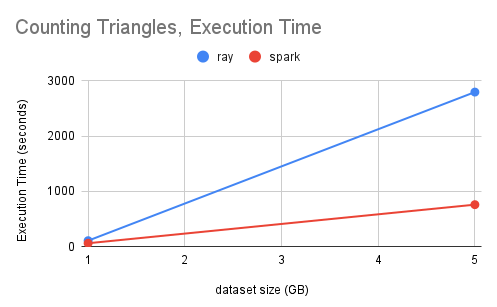
\includegraphics[width=0.9\columnwidth]{1}
\captionof{figure}{Spark is substantially faster than Ray for triangle
counting. As we can see in the graph, not only Ray is slower, but it
also has a greater slope which means their difference in execution time increases
with larger datasets.}


\end{figure}

\begin{figure}[H]\centering
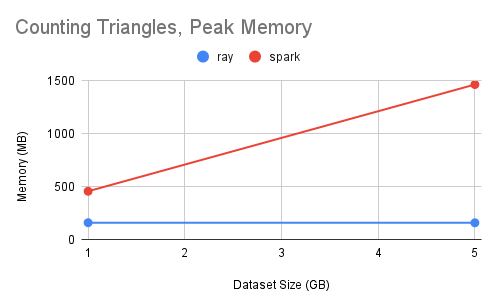
\includegraphics[width=0.9\columnwidth]{2}
\captionof{figure}{Spark uses more memory (peak) than Ray for
triangle counting.
Spark often achieves faster runtimes by caching intermediate data, such
as RDDs or DataFrames, in memory, reducing redundant recomputation but
raising peak memory usage \cite{zaharia2018spark, stackoverflow_cache}.
Ray, on the other hand, favors streaming and chunked data processing without extensive in-memory caching. Its Ray Data feature is designed for scalable, memory-efficient streaming and handles overflow by spilling to disk when necessary
\cite{ray_perf}.}
\end{figure}

\begin{figure}[H]\centering
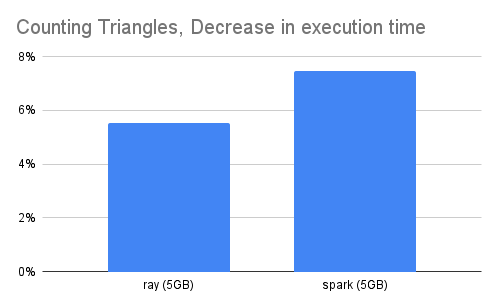
\includegraphics[width=0.9\columnwidth]{3}
\captionof{figure}{
Ray shows significantly more speedup than Spark when scaling from 2 to 3 workers for triangle counting. Spark showed almost no speed up, while Ray imporved by 17\%.}
\end{figure}

\begin{figure}[H]\centering
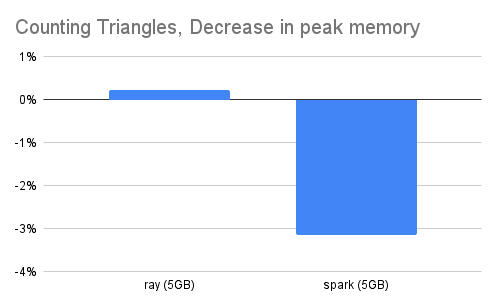
\includegraphics[width=0.9\columnwidth]{4}
\captionof{figure}{Scaling didn't significantly impact peak memory used by Ray or Spark for triangle counting,
as both had less than 1\% change when scaling from 2 to 3 workers.}
\end{figure}






%================ PageRank =================
\begin{figure}[H]
\centering
\captionof{table}{PageRank Benchmark Results}
\resizebox{0.9\columnwidth}{!}{%
\begin{tabular}{c c c c c c c}
\toprule
\multirow{2}{*}{Workers} &
\multicolumn{3}{c}{Time (s)} &
\multicolumn{3}{c}{Memory (MB)} \\ 
\cmidrule(lr){2-4} \cmidrule(lr){5-7}
 & Dataset (GB) & Ray & Spark & Dataset (GB) & Ray & Spark \\ 
\midrule
3 & 1 & 86.23 & 68.89 & 1 & 349.71 & 157.75 \\
3 & 5 & 475.92 & 184.18 & 5 & 999.91 & 174.69 \\
2 & 5 & 470.3 & 186.12 & 5 & 1000.09 & 165.84 \\
\bottomrule
\end{tabular}%
}
\end{figure}

\begin{figure}[H]\centering
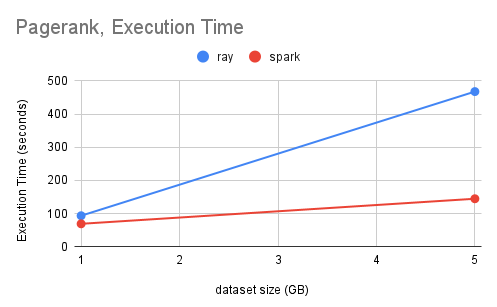
\includegraphics[width=0.9\columnwidth]{5}
\captionof{figure}{For PageRank, Spark is faster than Ray.}
\end{figure}

\begin{figure}[H]\centering
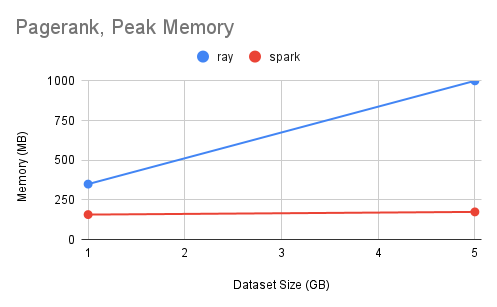
\includegraphics[width=0.9\columnwidth]{6}
\captionof{figure}{For PageRank, Spark also used less memory.
Spark's memory usage remains stable, while Ray's memory increases with dataset size.}
\end{figure}

\begin{figure}[H]\centering
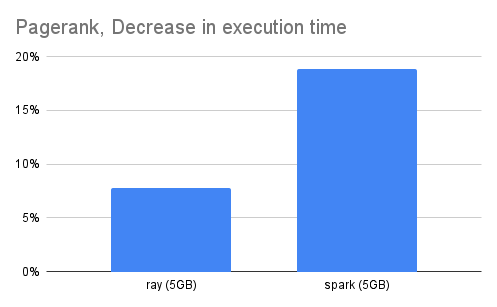
\includegraphics[width=0.9\columnwidth]{7}
\captionof{figure}{Scaling didn't significantly impact execution time for Ray or Spark for PageRank,
as both had less than 2\% change when scaling from 2 to 3 workers.}
\end{figure}

\begin{figure}[H]\centering
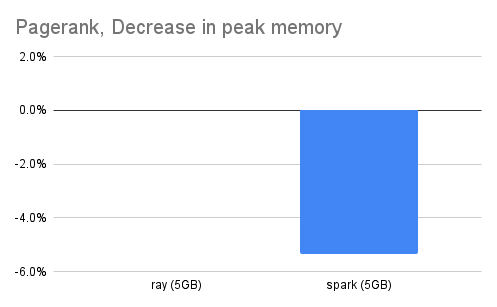
\includegraphics[width=0.9\columnwidth]{8}
\captionof{figure}{Scaling didn't significantly impact peak memory used by Ray, but increased
Spark's memory usage by 5\% when scaling from 2 to 3 workers.}
\end{figure}


\subsection{ETL}



%================ ETL Workloads =================
\begin{figure}[H]
\centering
\captionof{table}{ETL: Total (for Extract, Transform and Load) Benchmark Results}
\resizebox{0.9\columnwidth}{!}{%
\begin{tabular}{c c c c c c c}
\toprule
\multirow{2}{*}{Workers} &
\multicolumn{3}{c}{Time (s)} &
\multicolumn{3}{c}{Memory (MB)} \\ 
\cmidrule(lr){2-4} \cmidrule(lr){5-7}
 & Dataset (GB) & Ray & Spark & Dataset (GB) & Ray & Spark \\ 
\midrule
3 & 1 & 50.16 & 39.43 & 1 & 228 & 170.65 \\
3 & 5 & 261.5 & 204.95 & 5 & 229.18 & 166.87 \\
2 & 5 & 266.95 & 195.72 & 5 & 230.43 & 161.62 \\
\bottomrule
\end{tabular}%
}
\end{figure}

\begin{figure}[H]\centering
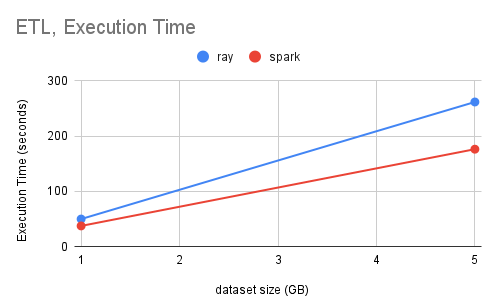
\includegraphics[width=0.9\columnwidth]{9}
\captionof{figure}{ETL: Execution time comparison. Spark is faster than Ray.}
\end{figure}

\begin{figure}[H]\centering
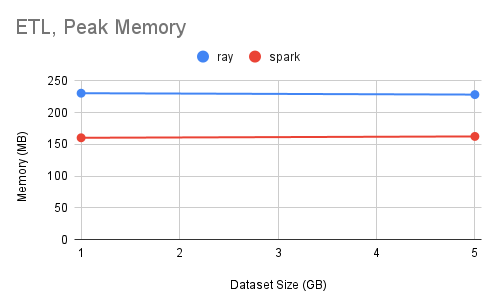
\includegraphics[width=0.9\columnwidth]{10}
\captionof{figure}{ETL: Memory usage comparison. Ray uses more memory than Spark. Both remain stable for larger datasets.}
\end{figure}

\begin{figure}[H]\centering
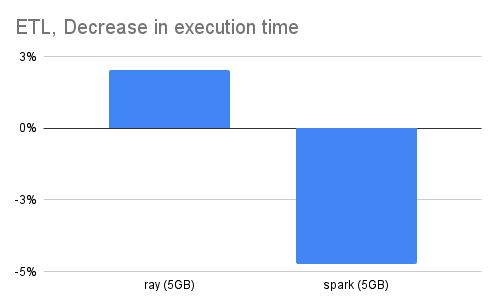
\includegraphics[width=0.9\columnwidth]{11}
\captionof{figure}{ETL: Scaling didn't significantly impact execution time for Ray or Spark,
as both had less than 5\% change when scaling from 2 to 3 workers.}
\end{figure}

\begin{figure}[H]\centering
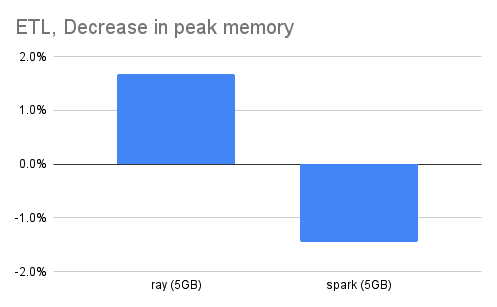
\includegraphics[width=0.9\columnwidth]{12}
\captionof{figure}{ETL: Scaling didn't significantly impact peak memory used by Ray or Spark.}
\end{figure}



% ETL Extract phase
\begin{figure}[H]
\centering
\captionof{table}{ETL Extract: Execution time for Ray and Spark}
\resizebox{0.9\columnwidth}{!}{%
\begin{tabular}{c c c c}
\toprule
Workers & Dataset (GB) & Ray & Spark \\ 
\midrule
3 & 1 & 15.05 & 23.53 \\
3 & 5 & 78.45 & 129.81 \\
2 & 5 & 80.08 & 124.1 \\
\bottomrule
\end{tabular}%
}
\end{figure}

\begin{figure}[H]\centering
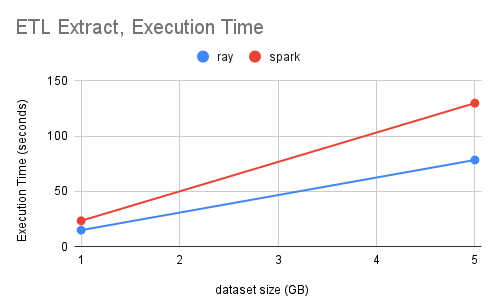
\includegraphics[width=0.9\columnwidth]{13}
\captionof{figure}{ETL Extract phase: Similar results, but Ray is faster.}
\end{figure}

\begin{figure}[H]\centering
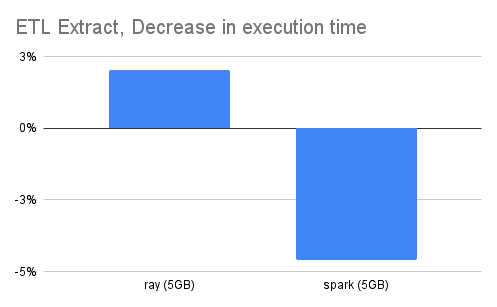
\includegraphics[width=0.9\columnwidth]{14}
\captionof{figure}{ETL Extract phase: Scaling didn't significantly impact execution time for Ray or Spark.}
\end{figure}

% ETL Transform phase
\begin{figure}[H]
\centering
\captionof{table}{ETL Transform: Execution time for Ray and Spark}
\resizebox{0.9\columnwidth}{!}{%
\begin{tabular}{c c c c}
\toprule
Workers & Dataset (GB) & Ray & Spark \\ 
\midrule
3 & 1 & 35.11 & 4.07 \\
3 & 5 & 183.05 & 19.15 \\
2 & 5 & 186.86 & 18.21 \\
\bottomrule
\end{tabular}%
}
\end{figure}

\begin{figure}[H]\centering
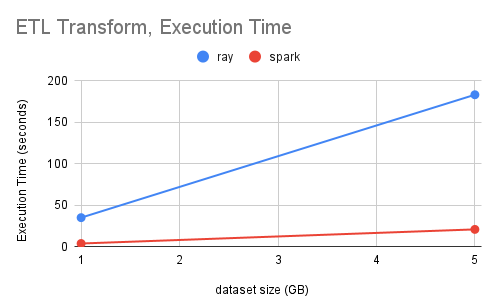
\includegraphics[width=0.9\columnwidth]{15}
\captionof{figure}{ETL Transform phase: Spark is substantially faster than Ray for Transform operations.}
\end{figure}


\begin{figure}[H]\centering
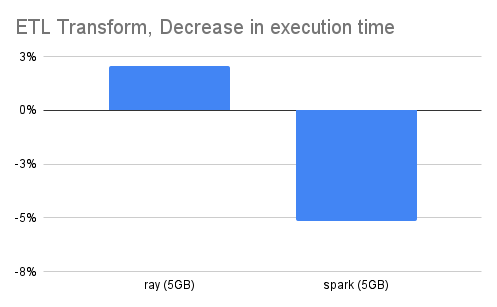
\includegraphics[width=0.8\columnwidth]{16}
\captionof{figure}{ETL Transform: Scaling didn't significantly impact peak memory used by Ray or Spark,
as both had less than 5.2\% change when scaling from 2 to 3 workers.}
\end{figure}


% ETL Load phase
\begin{figure}[H]
\centering
\captionof{table}{ETL Load: Execution time for Ray and Spark}
\resizebox{0.9\columnwidth}{!}{%
\begin{tabular}{c c c c}
\toprule
Workers & Dataset (GB) & Ray & Spark \\ 
\midrule
3 & 1 & 0 & 11.84 \\
3 & 5 & 0 & 56 \\
2 & 5 & 0 & 53.41 \\
\bottomrule
\end{tabular}%
}
\end{figure}

\begin{figure}[H]\centering
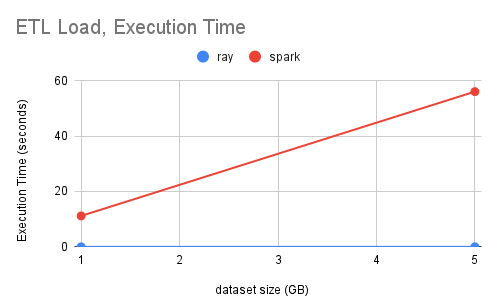
\includegraphics[width=0.9\columnwidth]{17}
\captionof{figure}{ETL Load phase: Ray reports negligible load time, likely attributable to in-memory operations, whereas Spark's load time increases with dataset size.}
\end{figure}

\begin{figure}[H]\centering
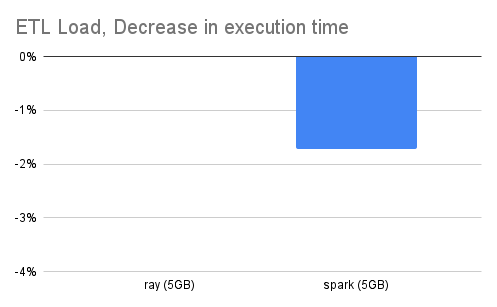
\includegraphics[width=0.9\columnwidth]{18}
\captionof{figure}{ETL Load phase: Scaling didn't significantly impact peak memory used by Ray or Spark.}
\end{figure}


\subsection{Machine Learning}


%================ Machine Learning =================
\begin{figure}[H]
\centering
\captionof{table}{k-means Benchmark Results}
\resizebox{0.9\columnwidth}{!}{%
\begin{tabular}{c c c c c c c}
\toprule
\multirow{2}{*}{Workers} &
\multicolumn{3}{c}{Time (s)} &
\multicolumn{3}{c}{Memory (MB)} \\ 
\cmidrule(lr){2-4} \cmidrule(lr){5-7}
 & Dataset (GB) & Ray & Spark & Dataset (GB) & Ray & Spark \\ 
\midrule
3 & 1 & 16.8 & 86.56 & 1 & 392.38 & 161.01 \\
3 & 5 & 196.72 & 285.34 & 5 & 724.59 & 161.56 \\
2 & 5 & 254.77 & 314.25 & 5 & 723.15 & 163.69 \\
\bottomrule
\end{tabular}%
}
\end{figure}

\begin{figure}[H]\centering
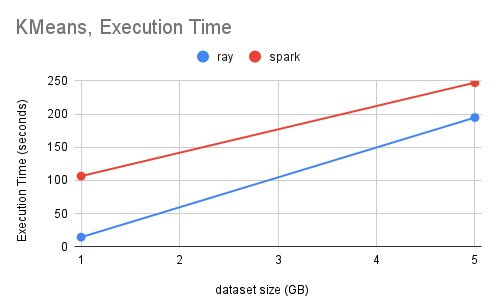
\includegraphics[width=0.9\columnwidth]{19}
\captionof{figure}{k-means: Ray is substantially faster for small datasets and remains faster than Spark for larger datasets too.}
\end{figure}


\begin{figure}[H]\centering
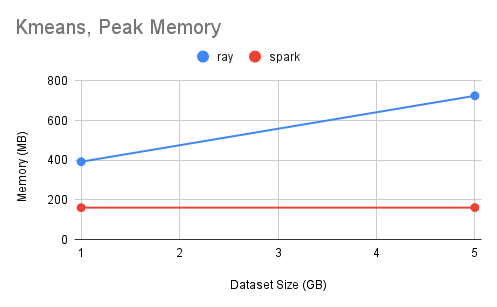
\includegraphics[width=0.9\columnwidth]{20}
\captionof{figure}{k-means: Spark used less memory than Ray.}
\end{figure}


\begin{figure}[H]\centering
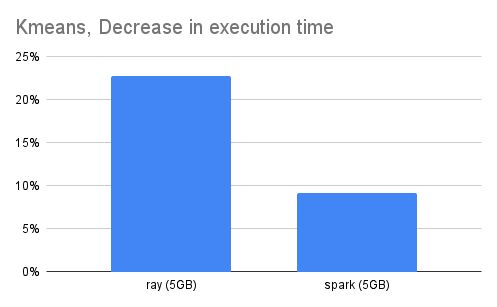
\includegraphics[width=0.9\columnwidth]{21}
\captionof{figure}{k-means: Both showed significant improvement in execution time when scaling,
but Ray improved by 23\% while Spark improved by 9\%.}
\end{figure}


\begin{figure}[H]\centering
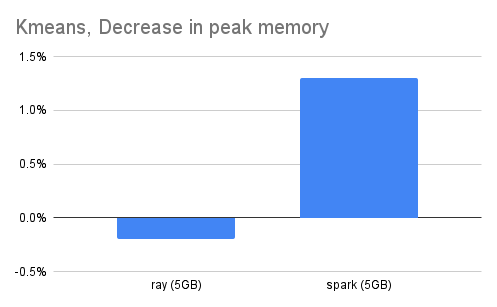
\includegraphics[width=0.9\columnwidth]{22}
\captionof{figure}{k-means: Scaling didn't significantly impact peak memory used by Ray or Spark.}
\end{figure}



\section{Comparison}

\subsection{Performance}

In graph processing workloads, Spark consistently outperforms Ray in
terms of execution time, reflecting its specialized graph processing
optimizations. Memory usage, however, depends on the specific
algorithm: Ray requires less memory for triangle counting, while
Spark is more memory-efficient for PageRank computations due to its
caching and shuffle strategies. In ETL workloads, each framework
demonstrates strengths in different phases. Spark achieves
substantially faster performance during the transformation phase,
leveraging in-memory operations and optimized data shuffles, but it
is relatively slower in data extraction and loading. In contrast,
Ray provides faster execution for machine learning tasks, though this
advantage comes with higher memory consumption. Overall, Spark offers
superior performance for graph operations and ETL transformations,
whereas Ray is more efficient for machine learning and ETL extraction
and loading phases. These results suggest a general trade-off:
frameworks that prioritize execution speed often incur higher memory
usage, while those optimizing memory tend to sacrifice some runtime
performance.


\subsection{Scalability}

The scaling experiments in this study were intentionally constrained to a small cluster expansion: 
increasing the number of worker nodes from 2 to 3. 
This represents a narrow scaling window and, while useful for illustrating relative framework behavior under modest additional parallelism, 
it does not permit strong generalization about multi-node scalability at larger scales (e.g., tens to hundreds of nodes). 
All observations below should therefore be interpreted as indicative within this limited regime rather than definitive statements about asymptotic scaling.


Ray scaled better in execution time for triangle counting and k-means clustering
because these workloads are highly parallelizable with minimal inter-worker communication,
allowing Ray’s fine-grained task scheduling to efficiently distribute work, but it showed
minimal change for PageRank, which involves iterative computations where each node depends
on its neighbors, so adding workers increases communication and synchronization overhead,
limiting scaling. Spark exhibited limited scaling benefits in execution time across all graph
workloads because its coarse-grained task scheduling and shuffle-heavy operations make graph
computations expensive, with only slight improvements for k-means, which can be more easily
parallelized. Both frameworks showed minimal improvement in ETL execution time when scaling
from 2 to 3 workers because these tasks are often I/O-bound, so adding workers does not reduce
the bottleneck. Overall, Ray performs better for CPU-bound, easily parallelizable tasks, while
communication-heavy or I/O-bound workloads see limited gains from additional workers in both
frameworks.

Neither Ray nor Spark reduced memory usage when scaling; peak memory stayed roughly the same, driven mainly by dataset size and computation rather than worker count.

A more comprehensive scalability characterization 
(e.g., strong and weak scaling across larger clusters, profiling shuffle and scheduling overheads, and exploring heterogeneous resources such as GPUs) 
is left to future work. Such experiments would help determine whether the relative advantages observed here persist, diminish, or invert under higher degrees of parallelism.

\subsection{Ease of Use}
Both Ray and Spark provide high-level
APIs that simplify the development of
distributed data processing pipelines, though they
differ in abstraction and workflow management.
Ray was much easier to set up,
as it is installed as a Python
library and requires minimal configuration to
run, making it accessible for quick experiments
and small-scale workflows. Spark, in contrast,
needs substantial configuration, including cluster setup,
resource management, and environment tuning, which can
be time-consuming and challenging for new users.
Once configured, Spark provides optimized execution
and built-in task scheduling for large workloads,
but the initial setup overhead is significant.
Overall, Ray offers a faster and simpler
way to start distributed computations, whereas
Spark is more complex to initialize but
provides extensive optimizations for high-performance workloads.

\section{Availability and Reproducibility}
All experiments were performed on publicly available datasets and using
open-source versions of Ray and Spark. Scripts, configuration files, and
instructions for reproducing the experiments are provided in the supplementary
materials and a public repository (link omitted here). The experiments use
standardized benchmarks for PageRank, ETL, triangle counting, and k-means,
ensuring that the results can be independently verified and extended by other
researchers. Containerization and virtual environment specifications further
improve reproducibility.

The scripts, configuration files, and instructions for reproducing the experiments are available at our 
\href{https://github.com/liuminex/Big-Data-HDFS-Ray-vs-Spark}{GitHub repository}.



\section{Conclusion}
This study provides a comparative evaluation of Ray and Spark
across graph processing, ETL, and machine learning workloads.
Spark demonstrates superior performance in graph operations and
ETL transformation tasks, largely due to its optimized libraries,
in-memory caching, and efficient shuffle strategies. Ray, however,
exhibits advantages in machine learning workloads and the extraction
and loading phases of ETL, benefiting from its flexible task-based
execution model. Memory usage patterns indicate a trade-off:
frameworks that prioritize execution speed often incur higher
memory consumption, while memory-efficient frameworks may experience
slower runtimes. Both frameworks scale effectively with additional
computational resources, although Spark’s specialized optimizations
allow it to maintain a performance edge in certain workloads. 

Future work could extend this comparison to streaming workloads, 
larger clusters, and GPU-accelerated training to assess 
how architectural differences evolve under increased scale and heterogeneity.



\begin{thebibliography}{00}

\bibitem{hdfs} IBM, ``What is HDFS?,'' IBM. Available: \url{https://www.ibm.com/think/topics/hdfs}.

\bibitem{ray} Ray Project, “Overview - Ray 2.48.0”. Available: \url{https://docs.ray.io/en/latest/ray-overview/index.html}.

\bibitem{spark} Amazon Web Services, “What is Apache Spark?,”. Available: \url{https://aws.amazon.com/what-is/apache-spark/}.

\bibitem{kumar2018community} S. Kumar, W. L. Hamilton, J. Leskovec, and D. Jurafsky, ``Community interaction and conflict on the web,'' in \textit{Proc. of the 2018 World Wide Web Conference (WWW)}, pp. 933--943, 2018.

\bibitem{reddit_snap} S. Kumar, W.L. Hamilton, J. Leskovec, D. Jurafsky, ``Reddit Hyperlinks Dataset'' Stanford SNAP. Available: \url{https://snap.stanford.edu/data/soc-RedditHyperlinks.html}.

\bibitem{triangles} Neo4j, ``Triangle Count,'' Neo4j Graph Data Science. Available: \url{https://neo4j.com/docs/graph-data-science/current/algorithms/triangle-count/}.

\bibitem{pagerank} E. Roberts and K. Schroeder, ``The Google PageRank Algorithm,'' Stanford University CS54N. Available: \url{https://web.stanford.edu/class/cs54n/handouts/24-GooglePageRankAlgorithm.pdf}.

\bibitem{kmeans} C. Piech, ``K-Means,'' Stanford University CS221. Available: \url{https://stanford.edu/~cpiech/cs221/handouts/kmeans.html}.

\bibitem{kmeans++} D. Arthur and S. Vassilvitskii, ``k-means++: The Advantages of Careful Seeding,'' in \textit{Proc. of the 18th Annual ACM-SIAM Symposium on Discrete Algorithms (SODA)}, pp. 1027--1035, 2007. Available: \url{http://theory.stanford.edu/~sergei/papers/kMeansPP-soda.pdf}. 

\bibitem{zaharia2018spark} M. Zaharia, R. Xin, P. Wendell, T. Das, M. Armbrust, A. Dave, X. Meng, J. Rosen, S. Venkataraman, M. J. Franklin, A. Ghodsi, J. Gonzalez, S. Shenker, and I. Stoica, ``Apache Spark: A Unified Engine for Big Data Processing,'' \textit{arXiv:1804.10563}, 2018. Available: \url{https://arxiv.org/abs/1804.10563}.

\bibitem{stackoverflow_cache} Stack Overflow, ``Spark cache vs broadcast,'' Available: \url{https://stackoverflow.com/questions/38056774/spark-cache-vs-broadcast}.

\bibitem{ray_perf} Ray Project, ``Performance Tips for Ray Data,'' Available: \url{https://docs.ray.io/en/latest/data/performance-tips.html}.


\end{thebibliography}


\end{document}
